\chapter{Systematic uncertainties}
\label{chap:cpv:syst}

Three sources of systematic uncertainty are considered in this analysis: the
choice of model used to extract the \PLambdac\ and \APLambdac\ signal yields;
the failure of the kinematic weighting procedure to fully equalise the
\PLambdab, muon, and proton kinematics between the modes; and the breaking of
the assumption that the \PLambdac\ candidates originate from the \LbToLcmuX\
decay.
The effect of these on the measurement of \dACP\ will be discussed in this
\lcnamecref{chap:cpv:syst} and, where appropriate, systematic uncertainties
will be computed and assigned.

\section{Fit model}
\label{chap:cpv:syst:fit}

The models used for the signal and combinatorial background components in the
mass fits, presented in \cref{chap:cpv:prelim_fits,chap:cpv:araw}, do describe
the data well.
However, other functional forms may also describe the data well but give
different yields, which may change the value of \dACP\@.
To assess the extent to which different models can affect the measurement, the
yields are extracted using the method of sideband subtraction.

\subsection{Region definitions and method validity}
\label{chap:cpv:syst:fit:defs}

A sideband subtraction is applied to the data as a alternative method to
measure the \pKK\ and \ppipi\ signal yields in the charge-separated samples.

The signal region is defined as a window \SI{20}{\MeVcc} wide for the \pKK\
data and \SI{30}{\MeVcc} wide for \ppipi, centred on the nominal value of the
\PLambdac\ mass of \SI{2286.46}{\MeVcc}~\cite{PDG2014}.
The wider \ppipi\ window accounts for the wider signal shape, which is itself
due to the larger energy release, or $Q$ value, of the \ppipi\ decay.
The two sideband regions, each \SI{10}{\MeVcc} wide for \pKK\ and
\SI{15}{\MeVcc} wide for \ppipi, are chosen such that the centres are
$\pm\sfrac{3}{2}$ signal window widths away from the signal window centre.
The signal and sideband regions are shown in \cref{fig:cpv:syst:mass_windows},
with the 2012 magnet down data overlaid for reference.

The assumption of the sideband subtraction technique that the background
\ac{PDF} is linear is justified by the good description of the background by a
linear function in the nominal fits.
The lack of any visible physics backgrounds after the full selection described
in \cref{chap:cpv:selection} suggests that the sidebands are purely
combinatorial, and that no peaking structures are present in the signal region
other than the that of the signal.
Finally, the assumption that the signal contribution to the data in the
sidebands is negligible is checked using \ac{MC}, where \SI{0.7}{\percent} of
the \ppipi\ truth-matched signal data are in the sidebands, and for \pKK\ the 
fraction of \SI{0.3}{\percent}.
These fractions are much smaller than the relative statistical uncertainties on
the signal yields shown in
\cref{tab:cpv:prelim_fits:yields:pKK,tab:cpv:prelim_fits:yields:ppipi}, and so
the level of contamination is considered to be negligible.

\begin{figure}
  \begin{subfigure}[b]{0.5\textwidth}
    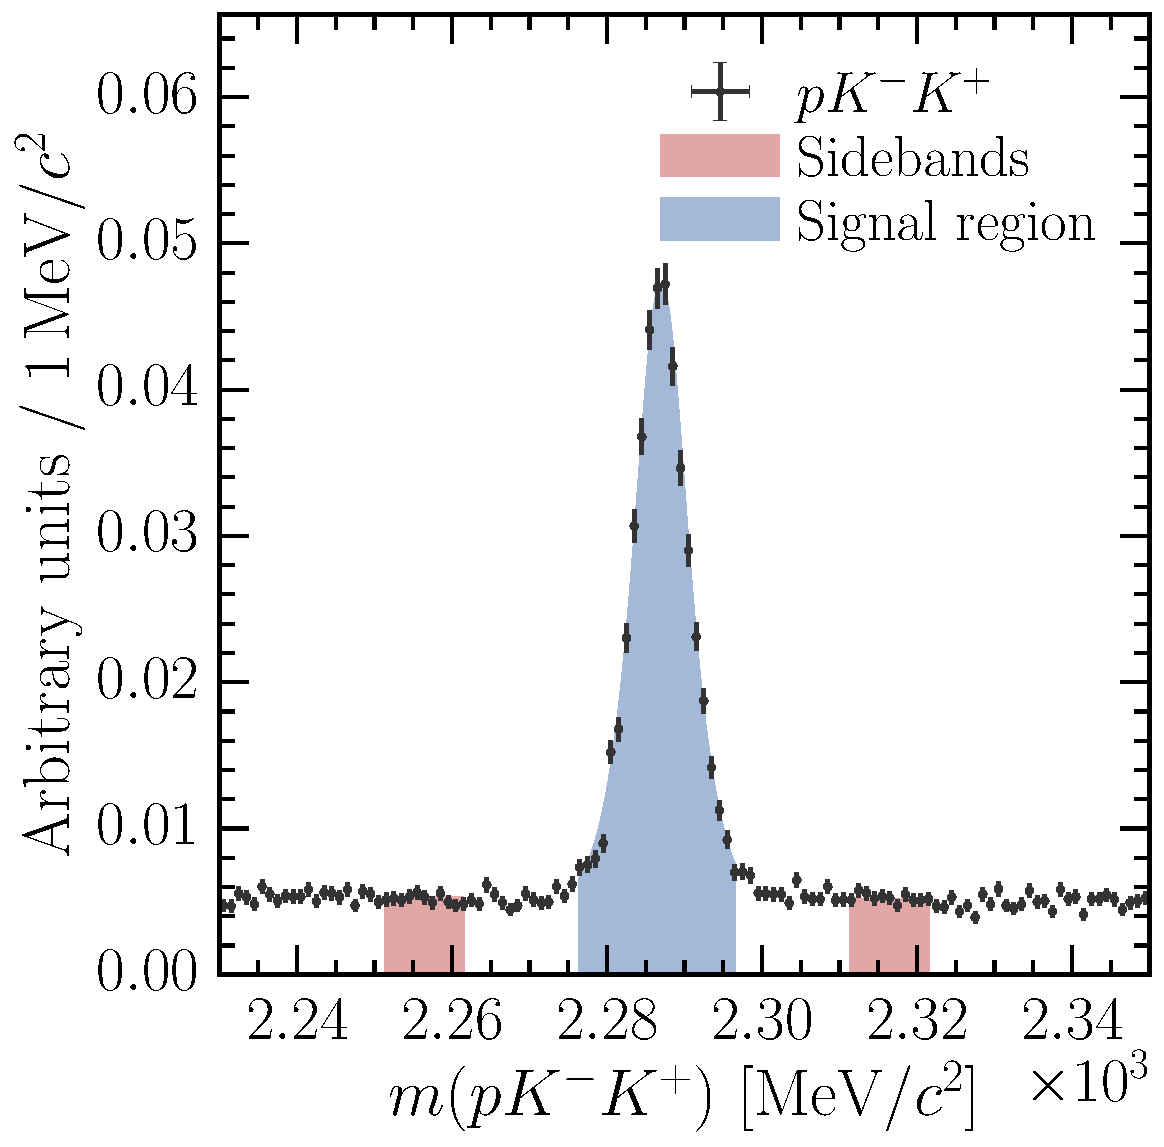
\includegraphics[width=\textwidth]{cpv/systematics/LcTopKK_2012_MagDown_Lb_DTF_Lc_M.pdf}
    \caption{\pKK}
    \label{fig:cpv:syst:mass_windows:pKK}
  \end{subfigure}
  \begin{subfigure}[b]{0.5\textwidth}
    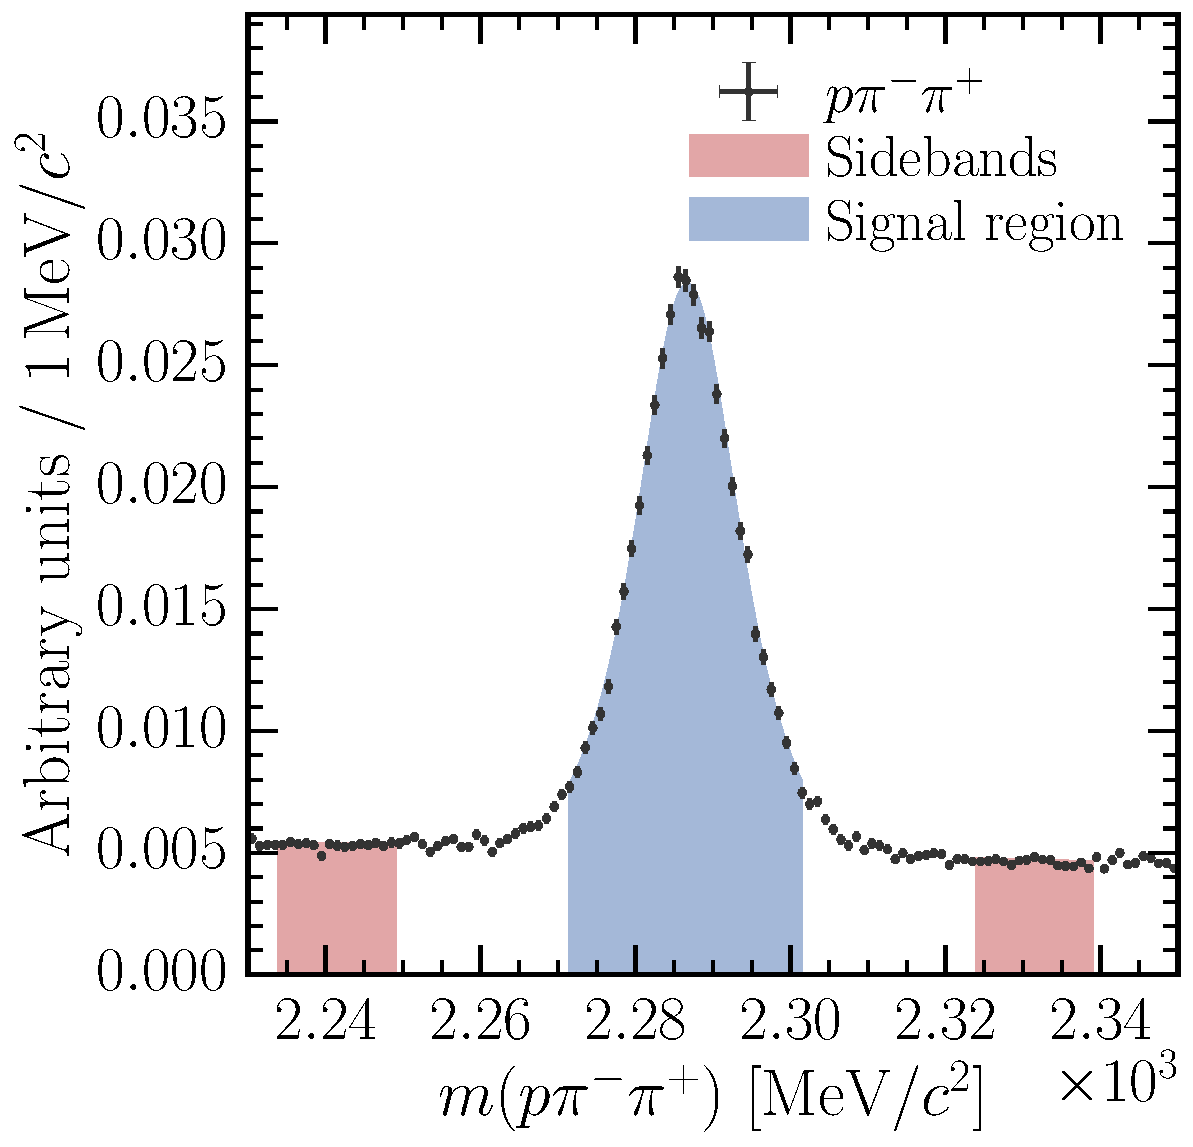
\includegraphics[width=\textwidth]{cpv/systematics/LcToppipi_2012_MagDown_Lb_DTF_Lc_M.pdf}
    \caption{\ppipi}
    \label{fig:cpv:syst:mass_windows:ppipi}
  \end{subfigure}
  \caption{%
    Definitions of the signal and sideband regions in the \PLambdac\ mass
    spectrum for \pKK~(\subref*{fig:cpv:syst:mass_windows:pKK}) and
    \ppipi~(\subref*{fig:cpv:syst:mass_windows:ppipi}).
    The 2012 magnet down data are overlaid for reference.
  }
  \label{fig:cpv:syst:mass_windows}
\end{figure}

\subsection{Results}
\label{chap:cpv:syst:fit:results}

For each data sub-sample, the \pKK\ and \ppipi\ samples are split by the charge
of the \PLambdac\ and the sideband subtraction technique is used to measure the
yields.
% TODO This should be the sum of the weights, rather than the candidate count
The yield asymmetry is then
\begin{equation}
  \ARaw(f) = \frac{%
    (N_{\text{S}}(\PLambdac) - N_{\text{SB}}(\PLambdac)) -
    (N_{\text{S}}(\APLambdac) - N_{\text{SB}}(\APLambdac))
  }{%
    (N_{\text{S}}(\PLambdac) - N_{\text{SB}}(\PLambdac)) +
    (N_{\text{S}}(\APLambdac) - N_{\text{SB}}(\APLambdac))
  },
  \label{eqn:cpv:syst:fit:araw_sb}
\end{equation}
where $N_{\text{S(SB)}}(\PLambdac)$ is the number of candidates in the signal
(sideband) region in the \PLambdac\ sample, and $N_{\text{S(SB)}}(\APLambdac)$
is the same but in the \APLambdac\ sample.
The counts are assumed to be Poisson-distributed, and so the uncertainty
$\unc{N}$ on each count is taken to be $\unc{N} = \sqrt{N}$.

The difference \dACP\ between \ARaw\ for \pKK\ and \ppipi\ is then computed
using the values obtain with \cref{eqn:cpv:syst:fit:araw_sb}, and the
difference is computed between those values and the nominal measurements given
in \cref{tab:cpv:results:asymmetries}.
The uncertainty on \ARaw\ is found by propagating the uncertainties on the
candidate counts using an \ac{MC} error propagation, and the values are assumed
to be fully correlated with those from the nominal procedure.
The differences for the measurements in all data sub-samples, and their
averages across years and magnet polarities, are presented in
\cref{tab:cpv:syst:sbs_differences}.
Almost all of the deviations from the nominal values are significant, and so
they taken as a systematic uncertainties on the measurements of \dACP\@.
The systematic uncertainty is \SI{0.26}{\percent} on the nominal result quoted
in \cref{eqn:cpv:results:dacp}.

\begin{sidewaystable}
  \centering
  \caption{%
    Differences between asymmetries measured with the nominal fit method and
    the sideband subtraction, measured for each data sub-sample and combination
    of sub-samples.
    The uncertainties quoted assume the values found by the two methods are
    fully correlated.
    The computation of the combinations, ``2011 + 2012'' and ``Average'', is
    defined in \cref{chap:cpv:results:combination}.
  }
  \label{tab:cpv:syst:sbs_differences}
  \begin{tabular}{ccS[table-format=2.2(2)]S[table-format=2.2(2)]S[table-format=2.2(2)]}
  \toprule
  Year & Polarity & {\ARaw(\pKK) (\si{\percent})} & {\ARaw(\ppipi) (\si{\percent})} & {\dACP (\si{\percent})} \\
  \midrule
2011 & Up & 0.73 \pm 0.06 & -0.95 \pm 0.21 & 1.68 \pm 0.03 \\
2011 & Down & -0.71 \pm 0.09 & -0.14 \pm 0.16 & -0.57 \pm 0.02 \\
2011 & Average & 0.01 \pm 0.05 & -0.55 \pm 0.13 & 0.56 \pm 0.01 \\
\midrule
2012 & Up & -0.00 \pm 0.06 & -0.29 \pm 0.14 & 0.28 \pm 0.01 \\
2012 & Down & 0.43 \pm 0.05 & 0.48 \pm 0.14 & -0.05 \pm 0.02 \\
2012 & Average & 0.21 \pm 0.04 & 0.10 \pm 0.10 & 0.12 \pm 0.01 \\
\midrule
$2011 + 2012$ & Up & 0.18 \pm 0.05 & -0.48 \pm 0.12 & 0.66 \pm 0.01 \\
$2011 + 2012$ & Down & 0.10 \pm 0.04 & 0.32 \pm 0.11 & -0.22 \pm 0.01 \\
$2011 + 2012$ & Average & 0.16 \pm 0.03 & -0.10 \pm 0.08 & 0.26 \pm 0.01 \\
  \bottomrule
\end{tabular}

\end{sidewaystable}

\section{Residual background asymmetries}
\label{chap:cpv:syst:asym}

The kinematic weighting discussed in \cref{chap:cpv:kinematic_weighting} does
not completely remove all differences between the \PLambdab, muon, and proton
kinematics between the \pKK\ and \ppipi\ datasets, nor does it remove all
\PKminus/\PKplus and \Ppiminus/\Ppiplus differences within the decay modes.
Therefore, contributions from the respective background asymmetries will still
contribute to \dACP\@.
A study is performed to quantity this contamination.
Firstly, the available measurements of the detection and production asymmetries
are enumerated, and then their application to this analysis is described.

The asymmetries considered are those that arise from the differences in the
matter and antimatter cross-sections with the detector, called detection
asymmetries.
The trigger asymmetry for muons from \Pbottom decays is known to be
small~\cite{Aaij:2016yze}, and is neglected here.

The pion detection asymmetry is measured using \sqrtseq{7}
data~\cite{Aaij:2012cy} by a method of partial reconstruction of
\PDstarp-tagged \decay{\PDzero}{\PKminus\Ppiplus\Ppiminus\Ppiplus} decays.
In this, the delta mass variable, defined similarly to that in
\cref{eqn:prod:fitting:delta_mass}, provides a good signal-to-background
discrimination even if the pion is not required to have been reconstructed.
The ratio of the signal yields before and after the explicit reconstruction
gives the pion detection efficiency, and this is performed separately for each
pion charge in bins of pion kinematics.
The asymmetries are shown in \cref{fig:cpv:syst:asym:pion} as a function of
pion momentum.
The central values of the relative asymmetries in bins of pion momentum are
small, generally less than \SI{2}{\percent}, and are very close to zero when
averaged across the magnet polarities.
The integrated ratios are measured to the $0.9914 \pm 0.0040$ and $1.0045 \pm
0.0034$ for magnet up and magnet down configurations, respectively.
Here, these values are considered to be compatible with zero, and so
contributions from a pion detection asymmetry are neglected.

The kaon detection asymmetry is measured using the full \runone\ dataset with
\DpToKpipi\ and \decay{\PDplus}{\APKzero\Ppiplus} decays~\cite{Aaij:2014gsa}.
The raw asymmetries between the two decays are subtracted, as is the
contribution from the $\APKzero$ interaction asymmetry, to measure \ADKpi.
The kaon material cross-section asymmetry is known to be much larger than that
for pions~\cite{PDG2014}, and so \ADKpi\ is assumed to be dominated by the kaon
detection asymmetry.
The asymmetry as a function of kaon momentum, averaged across magnet
polarities, is shown in \cref{fig:cpv:syst:asym:kaon}, where it is seen to be
significant larger in magnitude than the pion asymmetry in
\cref{fig:cpv:syst:asym:pion} and significantly different from zero.

The muon detection asymmetry is measured using the tag-and-probe technique described in \cref{chap:prod:effs:tracking} with \JpsiTomumu~\cite{Stahl:2010261}.
The track reconstruction efficiency is computed separately for \Pmuon and
\APmuon and an asymmetry is formed, shown in \cref{fig:cpv:syst:asym:muon}.
The asymmetries are small, of the order of \SI{0.1}{\percent}.

Measurements of the production asymmetry from unequal \PLambdab\ and
\APLambdab\ cross-sections have been made by \lhcb~\cite{Aaij:2015fea}, where
the asymmetry as a function of \pT\ was found to be negligible over both 2011
and 2012, but as a function of rapidity $\rapidity$ was found to be
\begin{equation}
  \APLb = (0.058 \pm 0.014)(y - \langle{y}\rangle),
\end{equation}
where $\langle{y}\rangle = 3.1$ is the average \PLambdab\ rapidity in the
sample used.
These values are compatible between the 2011 and 2012 data.
The same analysis also measured the proton detection asymmetry using
simulation, assigning a systematic uncertainty to the result based on the
relative disagreement between the data and the \ac{MC} when evaluating the
\emph{kaon} detection asymmetry.
The results are shown in \cref{tab:cpv:syst:asym:proton}.
Simulations using both the \pKK\ and the \ppipi\ samples defined in
\cref{chap:cpv:data:mc} agree with these results, and are shown in
\cref{fig:cpv:syst:asym:proton_this}.

\subsection{Evaluation}
\label{chap:cpv:syst:asym:eval}

The effect on the value of \dACP\ of the residual background asymmetry for a
single asymmetry $A$ due to some particle $X$ is given by a shift $\Delta{A}$,
defined as
\begin{equation}
  \Delta{A}^{X} = \frac{1}{\nsig^{\pKK}}\sum_{i} \nsig^{\pKK,i} A_{i} -
    \frac{1}{\nsig^{\ppipi}}\sum_{i} \nsig^{\ppipi,i} A_{i},
\end{equation}
where $\nsig^{f}$ is the total number of signal candidates in the \LcTof\ sample; $i$ is the bin index of the asymmetry parameter, such as \PLambdab\ rapidity; and $\nsig^{f,i}$ is the number of signal candidates in the \LcTof\ sample that fall in the $i$th asymmetry bin.
The number of signal candidates is computed as the sum of signal sWeights, weighted by kinematic weights and phase space efficiency corrections as in \cref{eqn:cpv:araw:total_weights}.
One such shift is defined for each of the muon and proton detection asymmetries
and the \PLambdab\ production asymmetry, $\Delta\APLb$, $\Delta\ADp$, and
$\Delta\ADmu$.
The shift due to the residual kaon detection asymmetry is similarly defined
\begin{equation}
  \Delta{\ADK} = \frac{1}{\nsig^{\pKK}}\left(%
    \sum_{i} \nsig^{\pKK,\PKminus} A_{i} -
    \sum_{i} \nsig^{\pKK,\PKplus} A_{i}
  \right),
\end{equation}
where $\nsig^{\pKK,\PKpm}$ is the number of signal \PKplus/\PKminus particles in the $i$th asymmetry bin.

The total shift of \dACP, $\Delta{A}$ is given by the sum of the individual shifts
\begin{equation}
  \Delta{A} = \Delta\APLb + \Delta\ADp + \Delta\ADmu + \Delta\ADK.
\end{equation}
These shifts for each year and data-taking condition are given in \cref{tab:cpv:syst:asym:results}, along with the shifts for the polarity-integrated datasets.
All of the values found are below one per mille, with the proton detection asymmetry providing the largest contribution.
Conservatively, a \SI{0.1}{\percent} systematic uncertainty is assigned to the measurement of \dACP\ based on the residual background uncertainty.

\begin{figure}
  \centering
  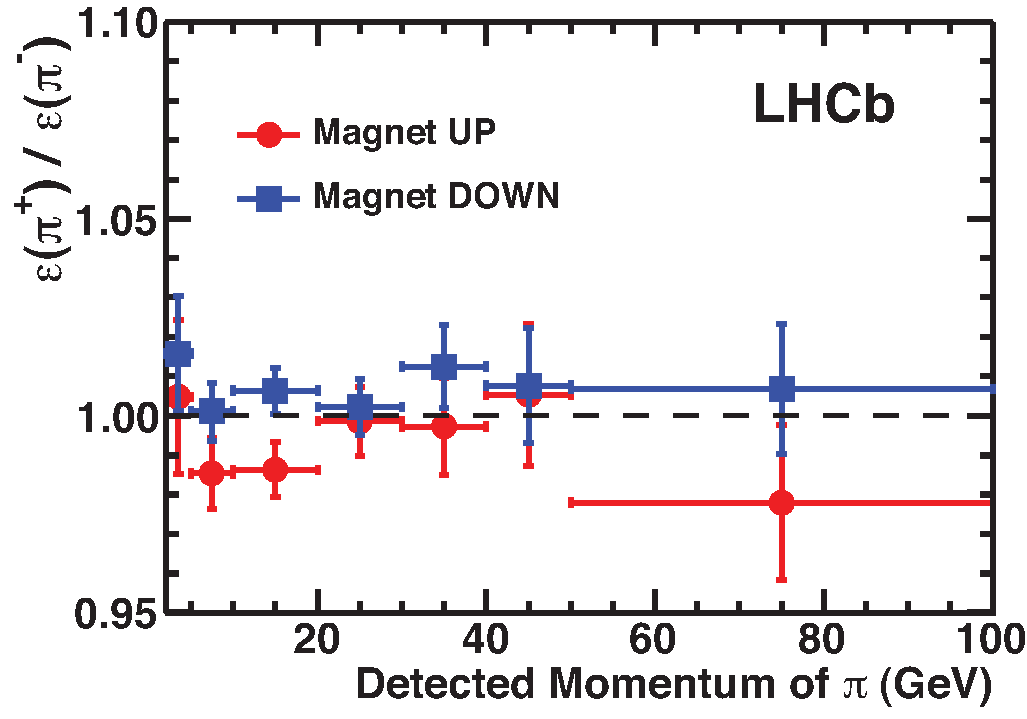
\includegraphics[width=0.75\textwidth]{cpv/systematics/pion_detection_asymmetry_p}
  \caption{%
    Ratio of pion detection asymmetries as a function of pion
    momentum~\cite{Aaij:2012cy}.
    The uncertainties on the data points are statistical.
  }
  \label{fig:cpv:syst:asym:pion}
\end{figure}

\begin{figure}
  \centering
  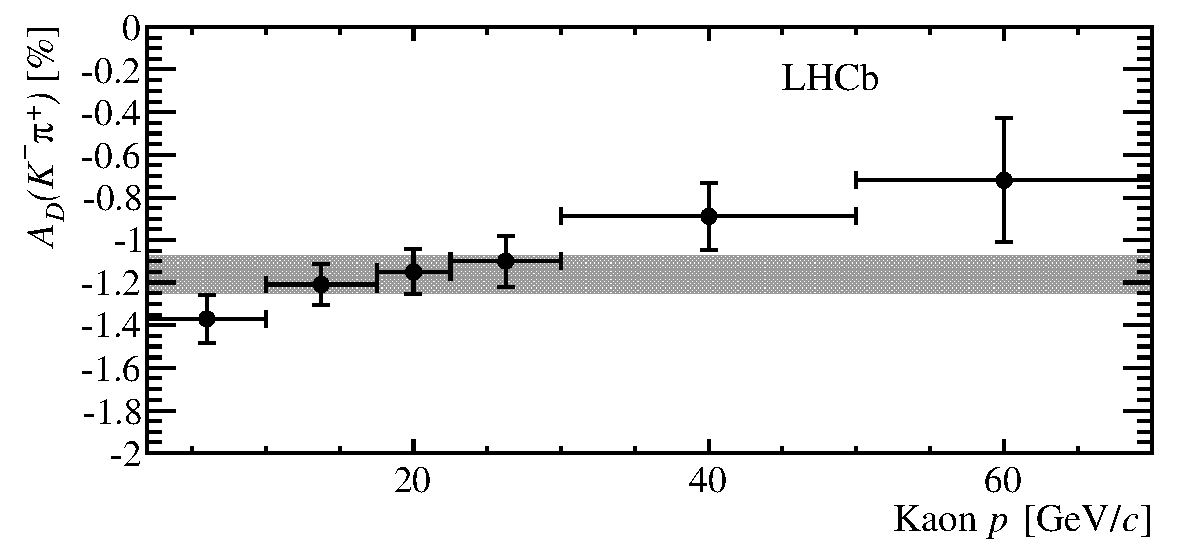
\includegraphics[width=\textwidth]{cpv/systematics/kaon_detection_asymmetry_p}
  \caption{%
    Kaon detection asymmetry \ADKpi\ as a function of kaon momentum averaged
    across magnet polarities~\cite{Aaij:2014gsa}.
    The average of the measurements is shown as a grey band.
    The error bars on the data points include statistical and systematic
    uncertainties.
  }
  \label{fig:cpv:syst:asym:kaon}
\end{figure}

\begin{figure}
  \centering
  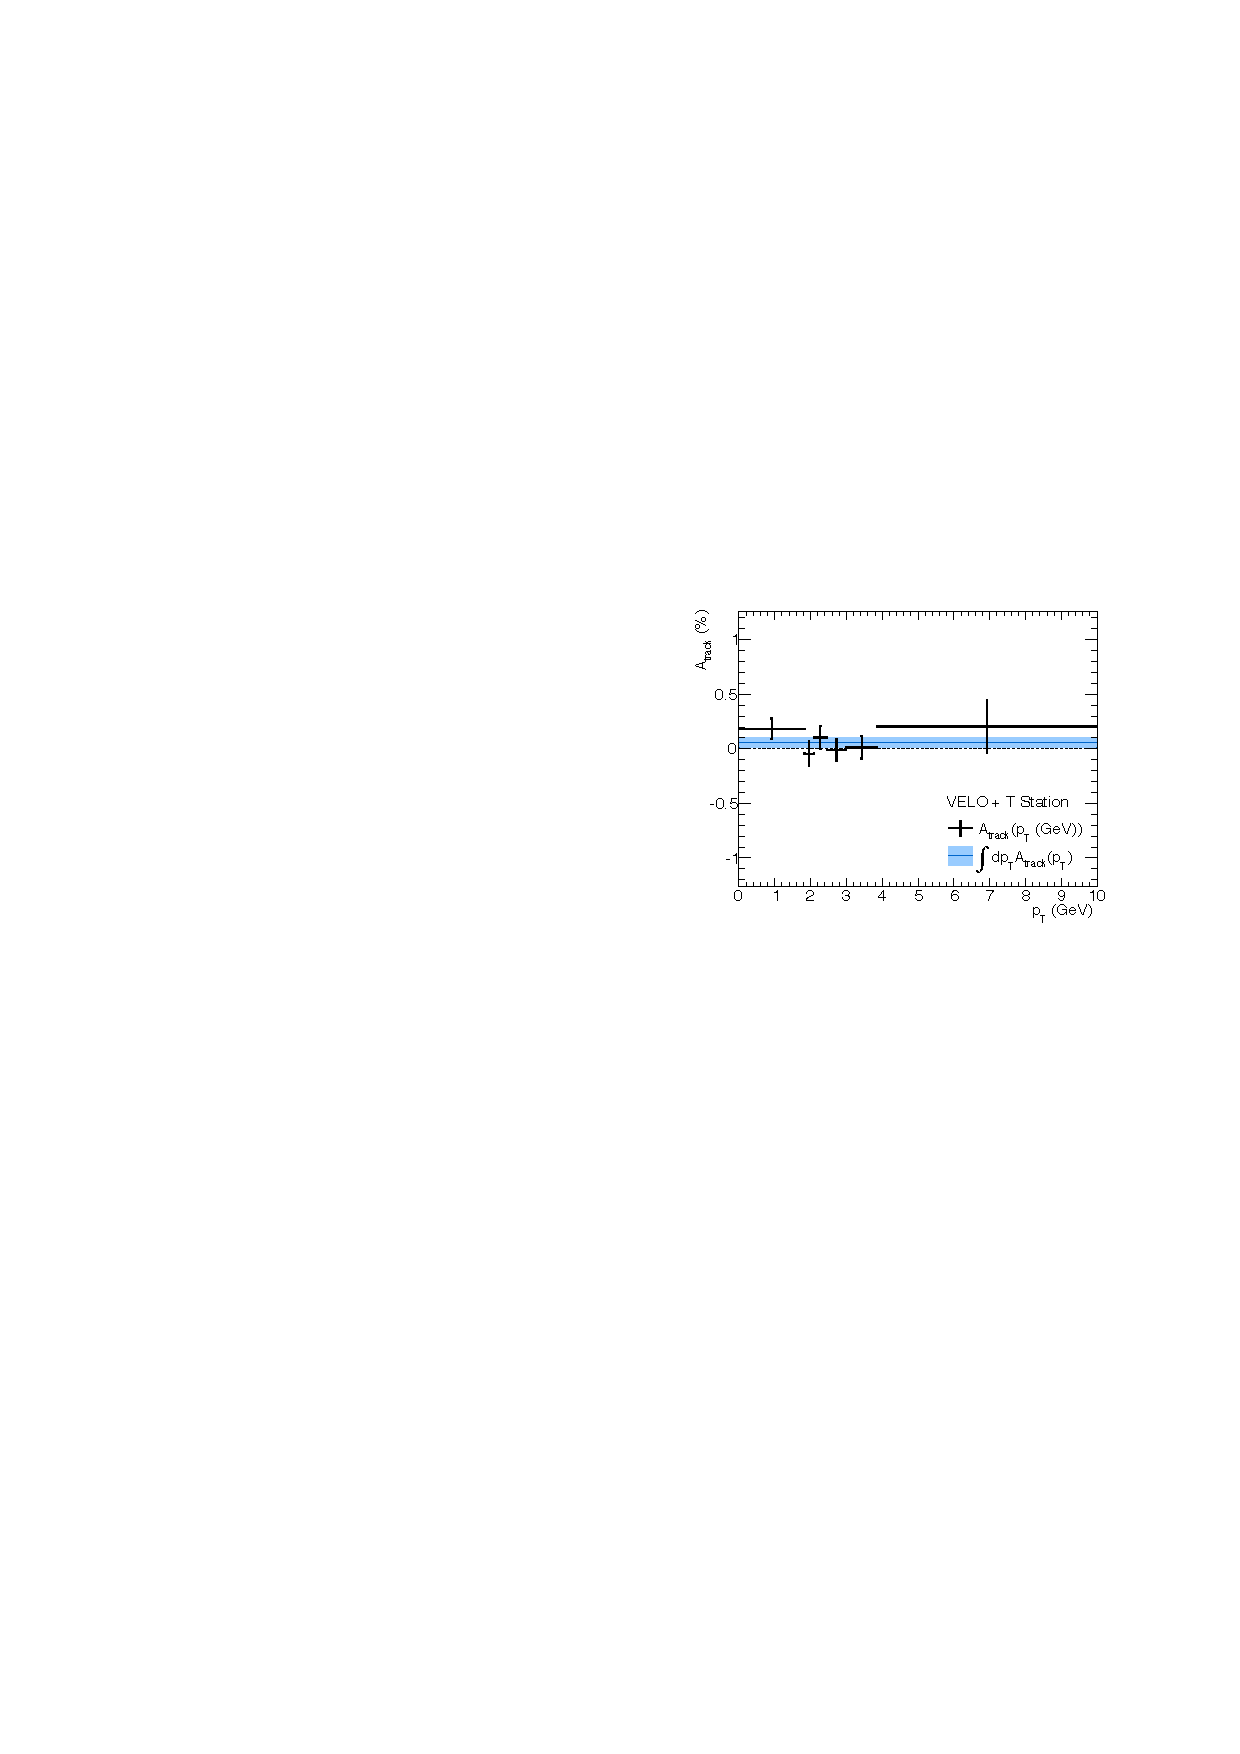
\includegraphics[width=0.75\textwidth]{cpv/systematics/muon_detection_asymmetry_pt}
  \caption{%
    Muon detection asymmetry as a function of muon \pT\ averaged
    across magnet polarities in \sqrtseq{8} data~\cite{Stahl:2010261}.
    The average of the measurements is shown as a blue band.
    The uncertainties on the data points are statistical.
  }
  \label{fig:cpv:syst:asym:muon}
\end{figure}

\begin{table}
  \centering
  \caption{%
    Proton detection asymmetries measured using simulation in bins of proton
    momentum~\cite{Aaij:2015fea}.
  }
  \label{tab:cpv:syst:asym:proton}
  \begin{tabular}{rclc}
  \toprule
  \multicolumn{3}{c}{Momentum bin [\si{\GeVc}]} & Asymmetry  [\si{\percent}] \\
  \midrule
  $0    $ & $< \ptot <$ & $10$   & 4.38 \pm 0.29  \\
  $10   $ & $< \ptot <$ & $17.5$ & 2.46 \pm 0.31  \\
  $17.5 $ & $< \ptot <$ & $22.5$ & 1.90 \pm 0.47  \\
  $22.5 $ & $< \ptot <$ & $30$   & 1.12 \pm 0.47  \\
  $30   $ & $< \ptot <$ & $50$   & 1.20 \pm 0.42  \\
  $50   $ & $< \ptot <$ & $70$   & 0.60 \pm 0.68  \\
  $70   $ & $< \ptot <$ & $100$  & -0.23 \pm 0.91 \\
  $100  $ & $< \ptot <$ & $150$  & 0.4 \pm 1.4    \\
  \bottomrule
\end{tabular}

\end{table}

\begin{figure}
  \centering
  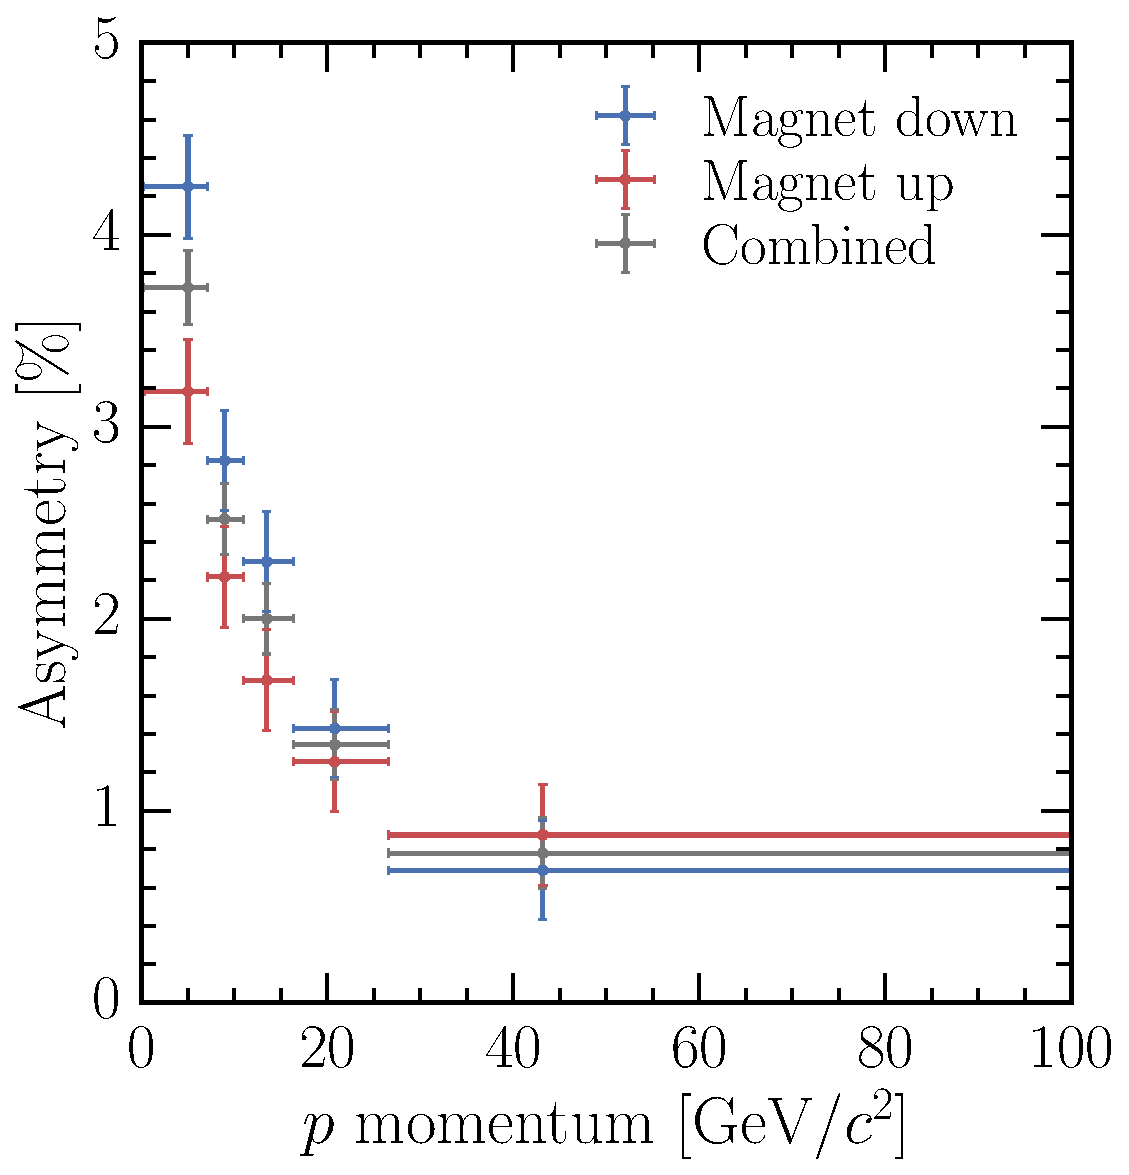
\includegraphics[width=0.75\textwidth]{cpv/systematics/proton_detection_asymmetry_p_this}
  \caption{%
    Asymmetry of the proton detection efficiency as a function of proton
    momentum in \si{\GeVc}.
    The uncertainties on the data points are statistical.
  }
  \label{fig:cpv:syst:asym:proton_this}
\end{figure}

\begin{sidewaystable}
  \centering
  \caption{%
    Shifts in the measurement of \dACP\ due to background asymmetries not
    complete removed during the kinematic weighting.
    The total shift $\Delta{A}$ is the sum of the individual ones, and all
    shifts are given in \num{e-4}.
  }
  \label{tab:cpv:syst:asym:results}
  \begin{tabular}{ccccccc}
  \toprule
  Year & Polarity & \APLb & \ADmu & \ADp & \ADK & $\Delta{A}$\\
  \midrule
  2011 & Up & $0.06 \pm 1.51$ & $0.35 \pm 0.44$ & $-7.08 \pm 1.13$ & $-0.00 \pm 0.00$ & $-6.68 \pm 1.93$ \\
  2011 & Down & $-0.97 \pm 1.62$ & $0.31 \pm 0.59$ & $-8.53 \pm 2.05$ & $-0.00 \pm 0.00$ & $-9.20 \pm 2.67$ \\
  2011 & Up+Down & $-0.68 \pm 1.07$ & $0.33 \pm 0.52$ & $-7.80 \pm 1.44$ & $-0.00 \pm 0.00$ & $-8.14 \pm 1.87$ \\
  \midrule
  2012 & Up & $0.56 \pm 0.82$ & $-0.05 \pm 0.16$ & $-6.84 \pm 1.19$ & $-0.00 \pm 0.00$ & $-6.33 \pm 1.45$ \\
  2012 & Down & $9.41 \pm 1.55$ & $-0.15 \pm 0.22$ & $-11.55 \pm 1.56$ & $-0.00 \pm 0.00$ & $-2.29 \pm 2.21$ \\
  2012 & Up+Down & $5.06 \pm 0.96$ & $-0.10 \pm 0.16$ & $-9.26 \pm 1.34$ & $-0.00 \pm 0.00$ & $-4.30 \pm 1.66$ \\
  \bottomrule
\end{tabular}

\end{sidewaystable}

\section{Signal decays from other sources}
\label{chap:cpv:syst:bkg}

The mass fits count the number of real \PLambdac\ decays in the samples.
However, backgrounds to \LbToLcmuX\ can peak in the \PLambdac\ mass spectrum,
such as baryonic decays of \PB\ mesons or promptly produced \PLambdac\ decays
associated with random muons.
These backgrounds will have different asymmetries, contaminating \dACP\@.

Selecting \pKK\ and \ppipi\ decays from promptly produced \PLambdac\ baryons
will contaminate \dACP\ with the \PLambdac\ production asymmetry.
\Cref{fig:cpv:syst:ipchisq} shows the signal \lnipchisq\ distributions in the
2012 magnet down data sample, in which a peaking structure corresponding to
prompt \PLambdac\ is not visible.
These distributions can be compared to the \lnipchisq\ distributions in samples
dominated by prompt charm, given in \cref{chap:prod:fitting}.
Even if there is a prompt \PLambdac\ component in the data used for the \dACP\
measurement, the contribution from a \PLambdac\ production asymmetry should
cancel as the \PLambdac\ kinematics are weighted to be equal.
To confirm this hypothesis, the data sample is split in two, defined by the
candidates passing or failing the cut $\lnipchisq > 4$.
The value of \dACP\ is recomputed for each sample, and the difference between
the two values is compatible with zero within \SI{1}{\sigma}.
No corresponding systematic uncertainty is assigned.

\begin{figure}
  \begin{subfigure}[b]{0.5\textwidth}
    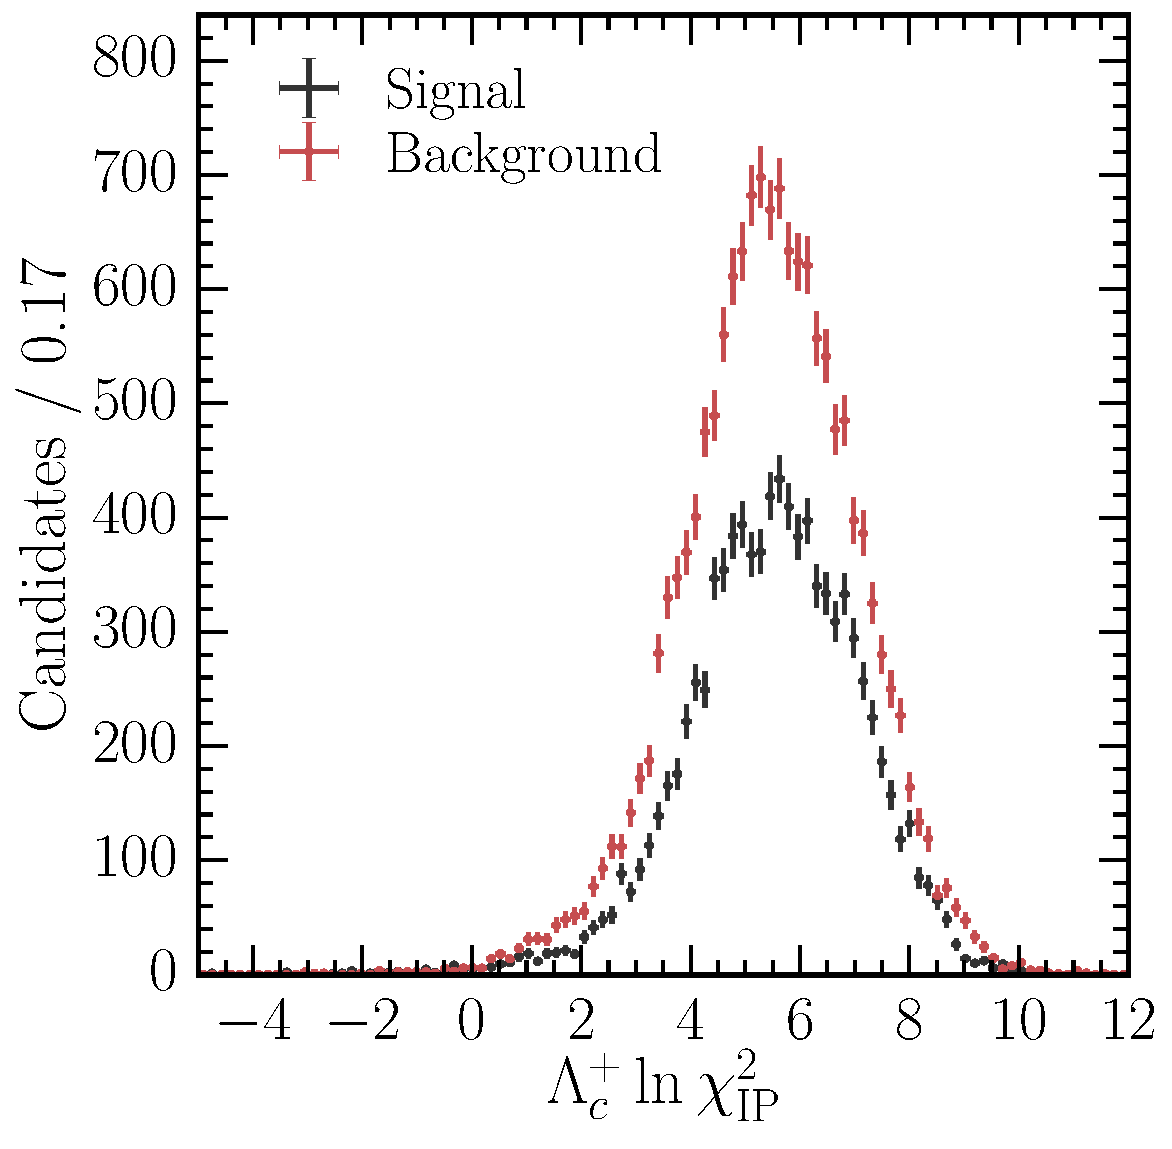
\includegraphics[width=\textwidth]{cpv/systematics/LcTopKK_2012_MagDown_Lc_IPCHI2_OWNPV.pdf}
    \caption{\pKK}
    \label{fig:cpv:syst:ipchisq:pKK}
  \end{subfigure}
  \begin{subfigure}[b]{0.5\textwidth}
    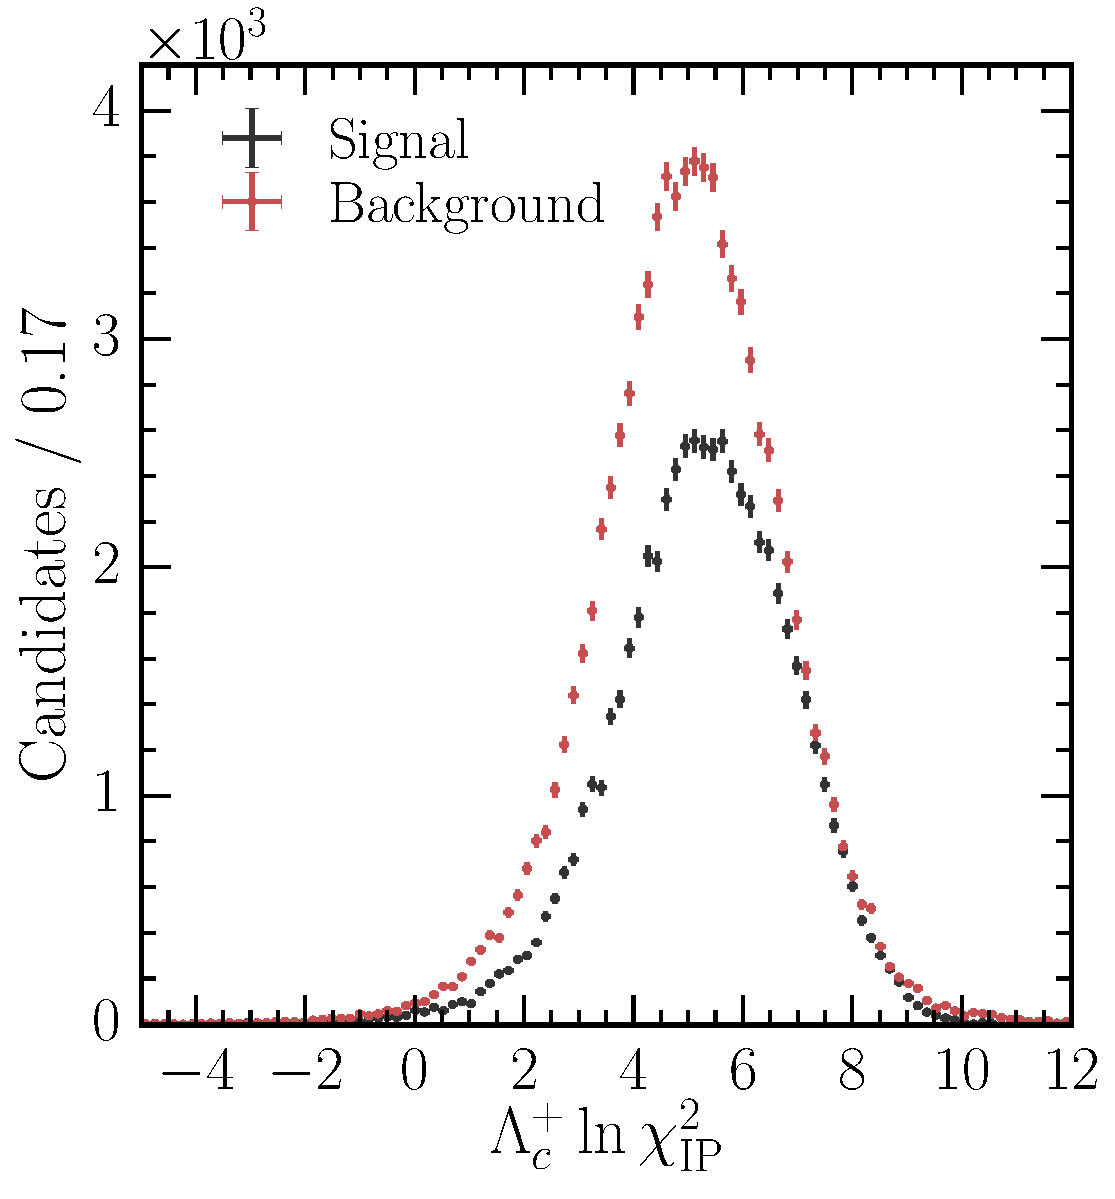
\includegraphics[width=\textwidth]{cpv/systematics/LcToppipi_2012_MagDown_Lc_IPCHI2_OWNPV.pdf}
    \caption{\ppipi}
    \label{fig:cpv:syst:ipchisq:ppipi}
  \end{subfigure}
  \caption{%
    Signal (black) and background (red) \lnipchisq\ distributions for
    \pKK~(\subref*{fig:cpv:syst:ipchisq:pKK}) and
    \ppipi~(\subref*{fig:cpv:syst:ipchisq:ppipi}) 2012 magnet down data
    samples.
    The \lnipchisq\ requirement made for the systematic studies is $\lnipchisq
    > 3$.
  }
  \label{fig:cpv:syst:ipchisq}
\end{figure}

Known alternative sources of \PLambdac\ from beauty decays are considered.
These include \decay{\PBplus}{\APLambdac\Pproton\Ppiplus} decays and
\decay{\PBplus}{\APSigmac\Pproton\Ppi\Ppi} with
\decay{\PSigmac}{\PLambdac\Ppi}.
In total, the inclusive \decay{\PB}{\PLambdac X} branching fractions are,
conservatively, less than \SI{10}{\percent} for both \PBplus and \PBzero, and
the \PBs contribution is negligible~\cite{PDG2014}.
The combined \PB cross-section is around four times that of the
\PLambdab~\cite{LHCb-PAPER-2013-004,Aaij:2015fea}, and the relative rate of
\decay{\PB}{\PLambdac X} is around 3 times that of \LbToLcmuX, for a total
relative rate of $N(\decay{\PB}{\PLambdac X})/N(\LbToLcmuX) = 12$.
However, the muon triggers and $\PLambdac\Pmuon$ vertex requirements strongly
suppress the alternate sources of \PLambdac\ decays.
In a simulated sample of one million generated
\decay{\PBzero}{\APLambdac\Pproton\Ppiminus\Ppiplus} decays, of the order of 10
\PLambdac\ candidates pass the selection requirements defined in
\cref{chap:cpv:selection}.
Given this, and that at least the \PBzero production asymmetry is compatible
with zero below the percent level~\cite{Aaij:2014bba}, the contribution from
\PB decays is neglected.

\section{Summary and combination}
\label{chap:cpv:syst:summary}

Sources of systematic uncertainties on the measurement of \dACP\ have been
studied.
The effect of the arbitrary choice of fit model is assessed with a sideband
subtraction method, with the deviation from the nominal result found to be
\SI{0.26}{\percent}.
Residual asymmetries arising from the failure of the kinematic weighting to
completely equalise all kinematic distributions are found to shift the value of
\dACP\ by \SI{0.1}{\percent}.
The contribution of \PLambdac\ candidates from non-\PLambdab\ decays is
considered to be negligible.

The two systematic uncertainties are added in quadrature in order to assign a
single systematic to \dACP, giving \SI{0.28}{\percent}.
This is small compared with the statistical uncertainty of \SI{0.89}{\percent}
given in \cref{tab:cpv:results:asymmetries}.
